%
% main.tex -- Paper zum Thema <thema>
%
% (c) 2018 Sebastain Lenhard und Nicolas Tobler, Hochschule Rapperswil
%
\chapter{Klima auf anderen Planeten\label{chapter:thema}}
\lhead{Klima auf anderen Planeten}
\begin{refsection}
\chapterauthor{Nicolas Tobler}

\section{Einleitung}

\begin{figure}
	% https://www.astrobio.net/news-exclusive/comparing-climates-from-earth-to-exoplanets/
  
	\centering
	\includegraphics[width=0.7\textwidth]{Pictures/planets.jpg}
	\caption{Mars, Erde und Venus massstabsgerecht}
\end{figure}

\rhead{Abschnitt}

%Verschiedene Organisationen, wie unter anderem Elon Musk's SpaceX, haben sich zum Ziel gemacht, in absehbarer Zukunft den Mars für den Menschen bewohnbar zu machen. Insbesondere sollte der Mars eine erdählnliche Atmosphere erhalte, also terraformed werden. Was auf Computer-generierten bildern ziemlich simpel aussieht, wird sich in realität wahrscheinlich ziemlich schwierig herausstellen. In diesem Kapitel wird die aktuelle lage des Klimas auf dem Mars analysiert und mögliche Wege den Mars zu teraformen auf die Machbarkeit untersucht.



venus co2 bindung
wie ist venus co geworden


was führt zu wasserlosen athmosphere
mars keine
venus ohne wasser
erde zwischendrin

boxmodell anteile element


%Grinspoon said, “It may be that conditions for life’s origin aren’t rare, but the hard part is the persistence of habitable conditions.”

\section{Das heutige Klima der Planeten}

Verschiedene Mars proben

\subsection{Temperatur}

\subsection{Albedo}

\subsection{Atmosphereische Eigenschaften}

dünne Atmosphere

Eann und wiso velohr der Mars seine Athmosphere


Rückgang der Atmosphere durch Sonnenwind
	https://www.nasa.gov/press-release/nasa-mission-reveals-speed-of-solar-wind-stripping-martian-atmosphere
	Vor 4.2 Milliarden Jahren gefrohr der Kern


\subsection{Treibhausgase}

wasser co2



Aussetzen von hocheffektiven treibhausgasen wie FCKW's

verwendung von Methan 




\section{Modell}

\begin{figure}
	\centering
	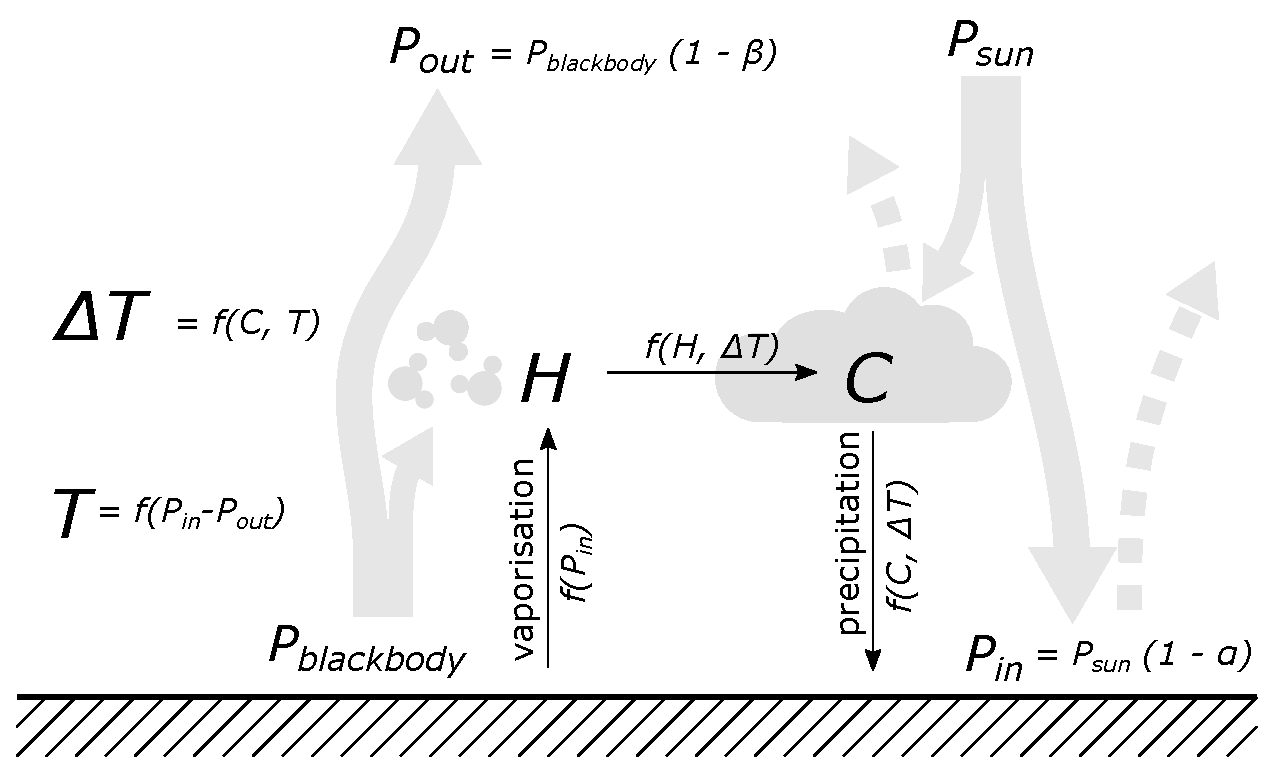
\includegraphics[width=\textwidth]{Pictures/Model.eps}
	\caption{Modell}
\end{figure}


Boxmodell

Parameter

atmosphere
wasser
co2
sauerstoff

land
wasser





\section{Energiehaushalt}

\begin{equation}
\dot{T} = P_{in} - P_{out}
\end{equation}

%reference to skript needed


\begin{equation}
P_{in} = \sigma T_{\astrosun}^4 \left( \frac{R_{\astrosun}}{a_{planet}} \right) ^2 \cdot (1-\alpha)
\end{equation}

$\alpha$ ist das albedo des Planeten.

\begin{equation}
P_{out} = (4 \pi R_{S}^2 \sigma T_{S}^4)(1 - \beta)
\end{equation}

$\beta$ ist der Treibhausfaktor

\subsection{Albedo}

Das albedo wird als Funktion der Wolkenabdeckung $C$ modelliert. Es wird ein linearer zusammenhang erwartet.

\begin{equation}
\alpha(C) = (0.65 \cdot C) + 0.15;
\end{equation}


Under der annahme, dass bei allen Planeten das Oberflächenbenalbedo gleich ist, wird ein minimales $\alpha_{min}$ und maximales Albedo $\alpha_{max}$ definiert. Bei 100\% Wolkendeckung soll der maximalwert erricht werden und bei 0\% der minimalwert.

\begin{equation}
\alpha = \alpha_{min} + C(\alpha_{max} - \alpha_{min})
\end{equation}

\subsection{Treibhauseffekt}

Wasserdampf ist ein sehr effektifes Treibhausgas. Es wird angenommen dass der atmosphärische Wasserdampf der Erde für 60\% des Treibhauseffekts sorgt.  

% 60\%    % https://www.acs.org/content/acs/en/climatescience/climatesciencenarratives/its-water-vapor-not-the-co2.html 



\begin{equation}
\beta(H) = 0.5 \cdot H
\end{equation}


\subsection{Wasserkreislauf}

Modellierung von atmosphärischem Wasserdampf $H$ als relative Luftfeuchtigkeit und Wolken $C$ als prozentuale Flächendeckung.


\subsubsection{Wasserdampfbildung}

Linearer zusammenhang zur Leistung

\begin{equation}
p_5 (P_{in})
\end{equation}

\subsubsection{Wolkenbildung}

\begin{equation}
p_6 \left( H \frac{dT}{dh} \right)
\end{equation}

Der Temperaturgradient wird als differenz der Oberflächentemperatur des Planeten und der Troposphärischen Temperatur modelliert. 

\begin{equation}
p_6 \left( H(T_S - T_T) \right)
\end{equation}

\subsubsection{Wolkenabbau}


\subsection{Zusammengefasst}


\begin{equation}
\dot{H} = p_5 (P_{in}) - p_4 \left( H(T_S - T_T) \right)
\end{equation}

\begin{equation}
\dot{C} = p_4 \left( H(T_S - T_T) \right) - p_5 C
\end{equation}


\subsection{Entweichen von atmosphärischen Gasen}

Ob ein Planet oder Mond eine Atmosphäre besitzt ist von wenigen parametern abhängig. Planeten behalten ihr Atmosphäre, wenn die Gravitation ausreichend stark ist, um die Moleküle gegen ihre thermische Geschwindigkeit zurückzuhalten.
Die Moleküle in der Atmosphäre, für die

% https://www.tcd.ie/Physics/people/Peter.Gallagher/lectures/PY4A03/pdfs/PY4A03_lecture12n13_amospheres.ppt.pdf

\begin{equation}
v_{escape} > v_{therm}
\end{equation}

zutrifft, werden nach und nach in den Weltraum abgestossen.
Die Fluchtgeschwindigkeit eines Planeten $v_{escape}$ wird durch deren Masse $M$ und Radius $R$ berechnet: 

\begin{equation}
v_{escape} = \sqrt{\frac{2GM}{R}}
\end{equation}

wobei $G$ die Gravitationskonstante ist. Die Fluchtgeschwindigkeit ist somit bei grossen und schweeren Gestirnen grösser.

Die thermische Geschwindigkeit eines Moleküls ist Maxwell-Bolzmann-verteilt. Deshalb gilt der berechnete Wert in diesem Zusammenhang nur approximativ. Die höchst wahrscheinliche Geschwindigkeit ist: 

\begin{equation}
v_{therm} = \sqrt{\frac{3kT}{m}}
\end{equation}

Dabei ist $k$ die Bolzmann-Konstante und $m$ die Mol-Masse des Moleküls. Die kritische Temperatur $T_{escape}$, bei welcher Gase abgestossen werden ist somit:

\begin{equation}
T_{escape} = \frac{2GMm}{3kR}
\end{equation}



\subsection{Differentialgleichung}

\begin{equation}
\left|
\begin{array}{lcl}
\dot{T}_T = p_1 \left( P_{in}(C) - P_{out}(T_S, H) \right) \\
\dot{T}_S = p_2 \left( P_{in}(C) \cdot H \right) - P_{blackbody}(T_T) - p_3 \left( (T_T - T_S) \cdot H \right) \\
\dot{C} = p_4 \left( H(T_S - T_T) \right) - p_5 C \\
\dot{H} = p_5 \left(P_{in} \right) - p_4 \left( H(T_S - T_T) \right)
\end{array}
\right|
\end{equation}

Um zu verhindern, dass eine Luftfeuchtigkeit oder Wolkenabdeckung von über 100\% auftritt, werden zu gewissen linearen Termen noch den gleichen Term mit grosser Potenz dazuaddiert. Somit wird der effekt verstärkt wenn die Grösse nahe an 100\% kommt.  

Mit Anpassungen für gesättigten Wasserdampf und wolkenabdeckung:

\begin{equation}
\left|
\begin{array}{lcl}
\dot{T}_T = p_1 \left( P_{in}(C) - P_{out}(T_S, H) \right) \\
\dot{T}_S = p_2 \left( P_{in}(C) \cdot H \right) - P_{blackbody}(T_T) - p_3 \left( (T_T - T_S) \cdot H \right) \\
\dot{C} = p_4 \left( (H + H^9)(T_S - T_T) \right) - p_5 (C + C^5) \\
\dot{H} = p_5 \left(P_{in} \right) - p_4 \left( (H + H^9 )(T_S - T_T) \right)
\end{array}
\right|
\end{equation}

\section{Ergebnisse}

Matlab plots



\section{Schlussfolgerung}
\rhead{Schlussfolgerung}

Abweichungen

Nicht modelierte faktoren:
chemische umwandlungen

\printbibliography[heading=subbibliography]
\end{refsection}
